\documentclass[../../main.tex]{subfiles}

\graphicspath{{\subfix{../../immagini/}}}

\begin{document}
    Come accade in un filtro di Bloom classico, anche l'obiettivo di un LBF è quello di memorizzare in modo efficiente in termini di spazio gli elementi, o chiavi, di un dato insieme, in questo capitolo chiamato $\mathcal{K}$, e di fornire la possibilità di controllare l'appartenenza di un generico elemento $x$ a tale insieme.

    La differenza rispetto al filtro base si trova nell'utilizzo di un classificatore per aiutare nel processo di controllo dell'appartenenza di un elemento all'insieme. Di fatto, il problema dell'appartenenza viene considerato come un problema di classificazione binaria in cui gli elementi appartenenti al filtro possiedono l'etichetta 1, mentre i rimanenti elementi possiedono etichetta 0.

    Più formalmente, l'obiettivo è quello di apprendere un modello $g$ in grado di predire correttamente la maggior parte degli elementi appartenenti all'insieme; il classificatore viene quindi addestrato su un training set $\mathcal{T}$ definito come unione degli insiemi $\mathcal{K}$, insieme delle chiavi, ed $\mathcal{U}$, insieme delle non-chiavi:
    \begin{equation}
        \mathcal{T} = \{(x_i, y_i = 1) | x_i \in \mathcal{K}\} \cup \{(x_i, y_i = 0) | x_i \in \mathcal{U}\}.
    \end{equation}
    Siccome la classificazione è di tipo binario, i modelli $g$ presi in considerazione sono reti neurali multistrato, il cui strato di output contiene un solo neurone con attivazione sigmoidale. Inoltre, la funzione di perdita $L$ da minimizzare prende il nome di log loss, e viene riportata di seguito:
    \begin{equation}
        L = \sum_{(x,y) \in \mathcal{T}}\left(y \log g(x) + (1 - y) \log(1 - g(x))\right).
        \label{eqn:logloss}
    \end{equation}
    Il valore $g(x)$ restituito dal modello rappresenta quindi la probabilità che l'elemento $x$ appartenga al filtro, si rende di conseguenza necessaria l'introduzione, per potere emettere come predizione un valore binario, di una soglia $\tau$. Un elemento verrà giudicato come appartenente al filtro se $g(x) > \tau$.
    
    Utilizzando solamente il classificatore però nasce la possibilità di ottenere dei falsi negativi: elementi $x \in \mathcal{K}$ per cui $g(x)$ risulta inferiore alla soglia, questo viola una delle caratteristiche fondamentali del filtro di Bloom, ovvero l'assenza di falsi negativi. Per eliminare i falsi negativi prodotti dal classificatore viene introdotto un filtro di backup, ovvero un filtro di Bloom incaricato di memorizzare tutti gli elementi appartenenti all'insieme $\mathcal{K}_{\tau}^- = \{x \in \mathcal{K} | g(x) < \tau\}$ dei falsi negativi.

    Infine, è utile per riassumere riportare la definizione di LBF data in \cite{10.5555/3326943.3326986}: 

    ``Un LBF $(g, \tau, B)$, definito su un insieme di chiavi $\mathcal{K}$ ed un insieme di non-chiavi $\mathcal{U}$, è una struttura composta da una funzione $g : \mathcal{X} \rightarrow [0,1]$, dove $\mathcal{X}$ è l'insieme universo, una soglia $\tau$, e da un filtro di Bloom $B$, chiamato filtro di backup, il cui compito è salvare tutti gli elementi dell'insieme $\mathcal{K}_{\tau}^- = \{x \in \mathcal{K} | g(x) < \tau\}$, ovvero l'insieme di falsi negativi generati da $g$. Dato un qualsiasi elemento $x$, l'LBF ritorna $x \in \mathcal{K}$ se $g(x) > \tau$ o se $g(x) < \tau$ e il filtro di backup ritorna $x \in \mathcal{K}$. In tutti gli altri casi l'LBF ritorna $x\notin \mathcal{K}$.''

    La Figure \ref{fig:BFInizializzazione} e \ref{fig:LBFInizializzazione} mettono a confronto la procedura di inizializzazione per le due tipologie di filtro presentate. Nello specifico, la Figura \ref{fig:BFInizializzazione} mostra l'inizializzazione per un filtro di Bloom, mentre la Figura \ref{fig:LBFInizializzazione} quella di un LBF.

    \begin{figure}[H]
        \centering
        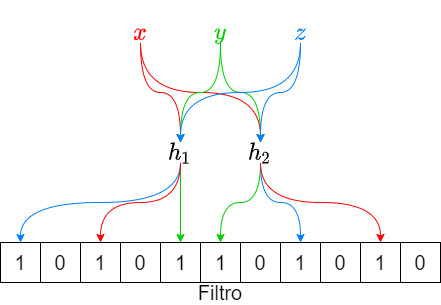
\includegraphics[width=\textwidth]{immagini/5_1/BFInizializzazione.png}
        \caption{Procedura di inizializzazione di un filtro di Bloom: tutti gli elementi dell'insieme $\mathcal{K}$ vengono passati attraverso le funzioni di hash $k$, e i bit presenti nelle posizioni corrispondenti ai risultati ottenuti vengono posti ad 1.}
        \label{fig:BFInizializzazione}
    \end{figure}

    \begin{figure}[H]
        \centering
        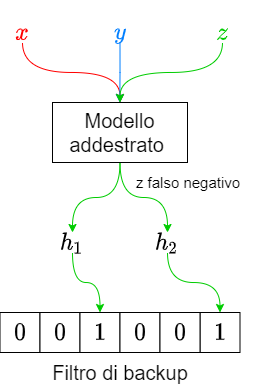
\includegraphics[width=\textwidth/2]{immagini/5_1/LBFInizializzazione.png}
        \caption{Procedura di inizializzazione di un LBF: tutti gli elementi dell'insieme $\mathcal{K}$ vengono passati attraverso il modello addestrato sul dataset $\mathcal{T}$, se un elemento viene etichettato come negativo viene inserito nel filtro di backup.}
        \label{fig:LBFInizializzazione}
    \end{figure}
\end{document}